\chapter{Résultats et bilan}
\label{chap:resultats}

\agtlettrine{C}e dernier chapitre dresse le bilan du projet : les
résultats obtenus domaine par domaine, un parcours applicatif de bout en
bout illustrant leur articulation, un aperçu visuel de l'application,
les tests de validation effectués, puis les limites actuelles et les
risques assumés à ce jour.
\minisommaire

\section{Résultats obtenus}

Le tableau~\ref{tab:resultats-domaines} reprend, sous une forme
condensée, la synthèse des quatorze domaines fonctionnels déjà détaillée
au chapitre~\ref{chap:etude-technique}, confirmée par l'implémentation
réalisée au chapitre~\ref{chap:realisation}.

\begin{table}[H]
\centering
\small
\renewcommand{\arraystretch}{1.3}
\begin{tabular}{p{5.5cm}p{8cm}}
\toprule
\textbf{Domaine} & \textbf{Résultat} \\
\midrule
Serveurs physiques et connectivité SSH & Réalisé \\
Conteneurs Docker et registres privés & Réalisé \\
Environnements & Réalisé \\
Console web & Réalisé \\
Diagnostic à la demande et alertes & Réalisé \\
Supervision continue & Réalisé \\
Déploiement continu & Réalisé \\
Publication applicative & Réalisé \\
Sauvegardes & Non réalisé \\
Montée en charge & Non réalisé \\
Contrôle d'accès dynamique & Réalisé \\
Sécurité & Non réalisé \\
Journal d'audit & Traçabilité réalisée, écran dédié non branché \\
Documentation intégrée & Réalisé \\
\bottomrule
\end{tabular}
\caption{Synthèse des résultats par domaine}
\label{tab:resultats-domaines}
\end{table}

\section{Parcours applicatif de bout en bout}

Le diagramme d'activité de la figure~\ref{fig:workflow-e2e} illustre
l'articulation complète de trois modules, présentés séparément aux
chapitres précédents : brancher un serveur, y déployer une application,
puis la publier publiquement sous un nom de domaine, en HTTPS.

\begin{figure}[H]
  \centering
  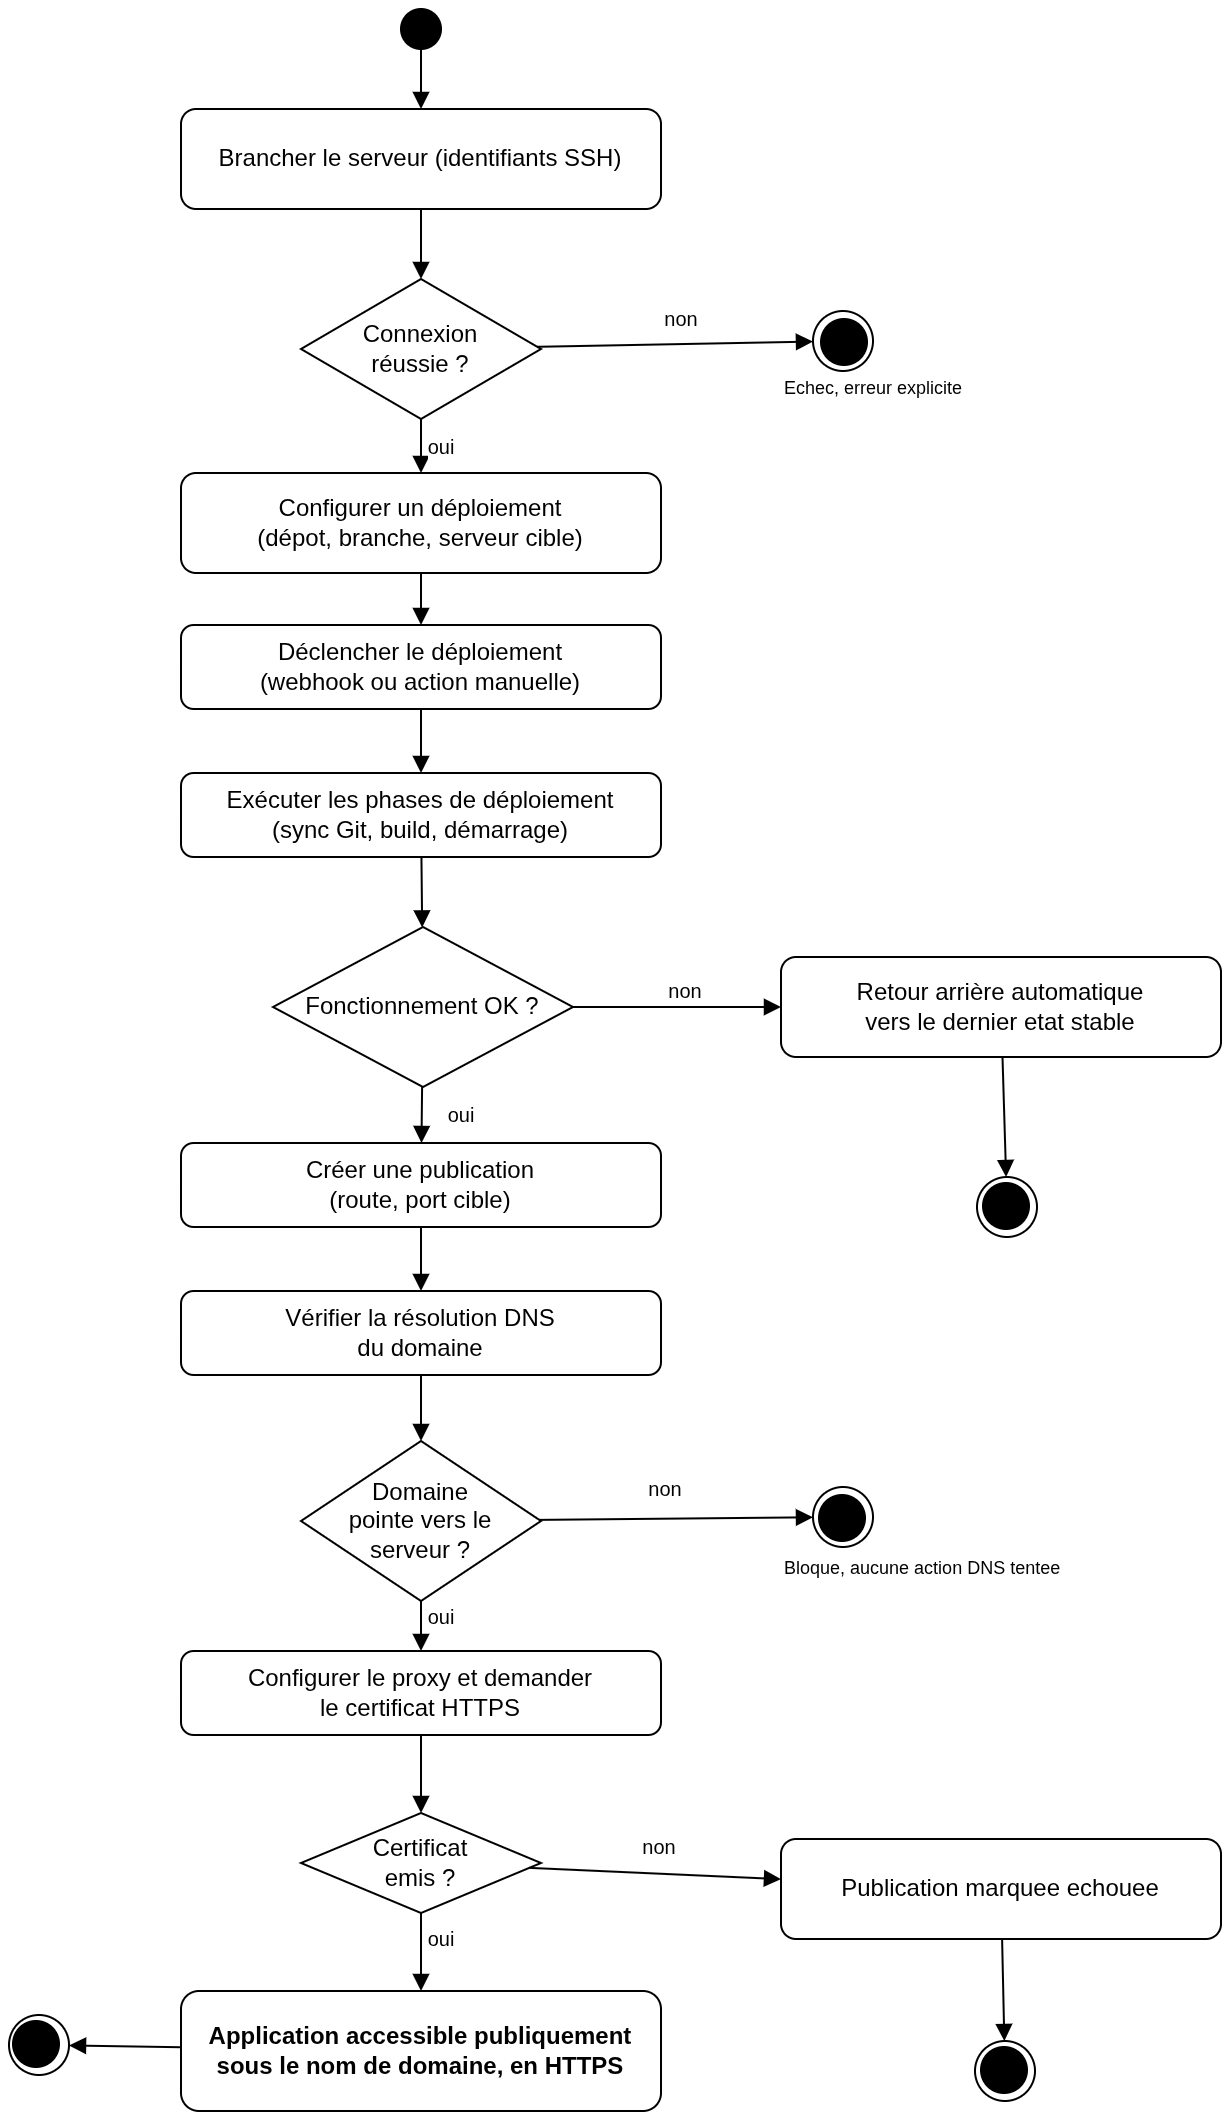
\includegraphics[width=0.85\linewidth]{assets/diagrams/05-diagramme_activite_deploiement_publication.png}
  \caption{Parcours de bout en bout : brancher, déployer, publier}
  \label{fig:workflow-e2e}
\end{figure}

Ce parcours met en évidence un principe déjà énoncé au
chapitre~\ref{chap:etude-technique} : aucune étape n'est corrigée
automatiquement en cas d'échec. Une connexion SSH refusée, un domaine
mal résolu ou un certificat non émis interrompent le parcours avec un
message explicite, plutôt que de tenter une correction silencieuse.

\section{Aperçu de l'application}

Les captures suivantes illustrent l'interface réelle d'AGT Infra, sur
les écrans les plus représentatifs des domaines déjà détaillés dans ce
rapport.

Le tableau de bord donne une vue d'ensemble immédiate du parc : nombre
de serveurs connectés, conteneurs actifs, pipelines de déploiement en
cours, applications en erreur et alertes actives, avec un état détaillé
par serveur.

\begin{figure}[H]
  \centering
  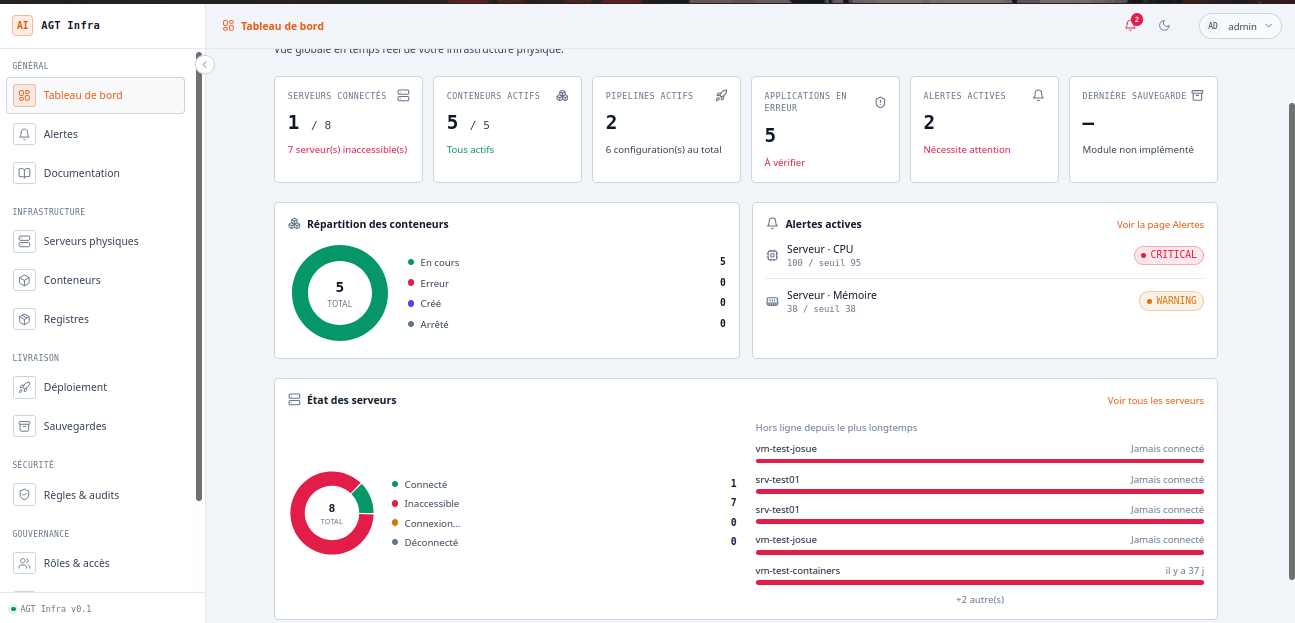
\includegraphics[width=0.85\linewidth]{assets/screenshots/05-screenshot_tableau_de_bord.png}
  \caption{Tableau de bord}
\end{figure}

L'écran de gestion des rôles et des accès liste les membres de l'équipe,
le rôle qui leur est affecté, ainsi que les permissions directes
accordées ou refusées à une personne précise, avec leur portée
(ressource concernée) et leur statut ALLOW ou DENY.

\begin{figure}[H]
  \centering
  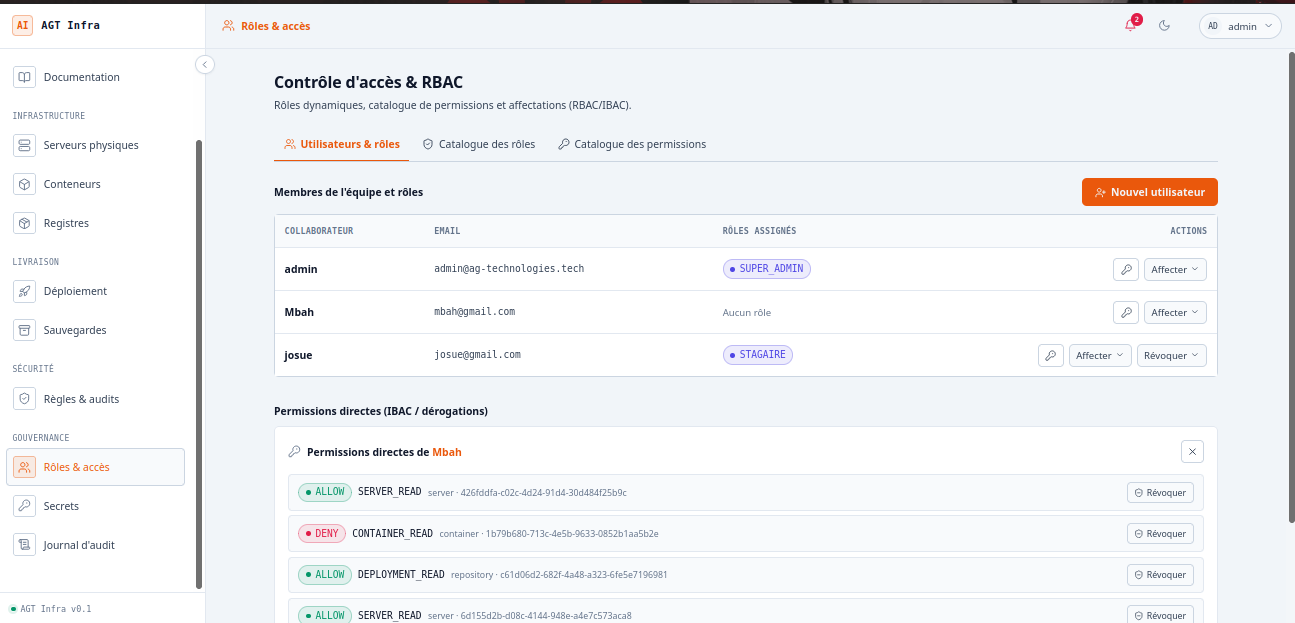
\includegraphics[width=0.85\linewidth]{assets/screenshots/05-screenshot_catalogue-de-membre-avec-permission.png}
  \caption{Gestion des rôles et des permissions directes}
\end{figure}

Ce formulaire illustre l'octroi d'une permission directe : la
permission concernée, son statut, sa portée restreinte à une ressource
précise plutôt que globale, et un motif obligatoire justifiant cette
dérogation.

\begin{figure}[H]
  \centering
  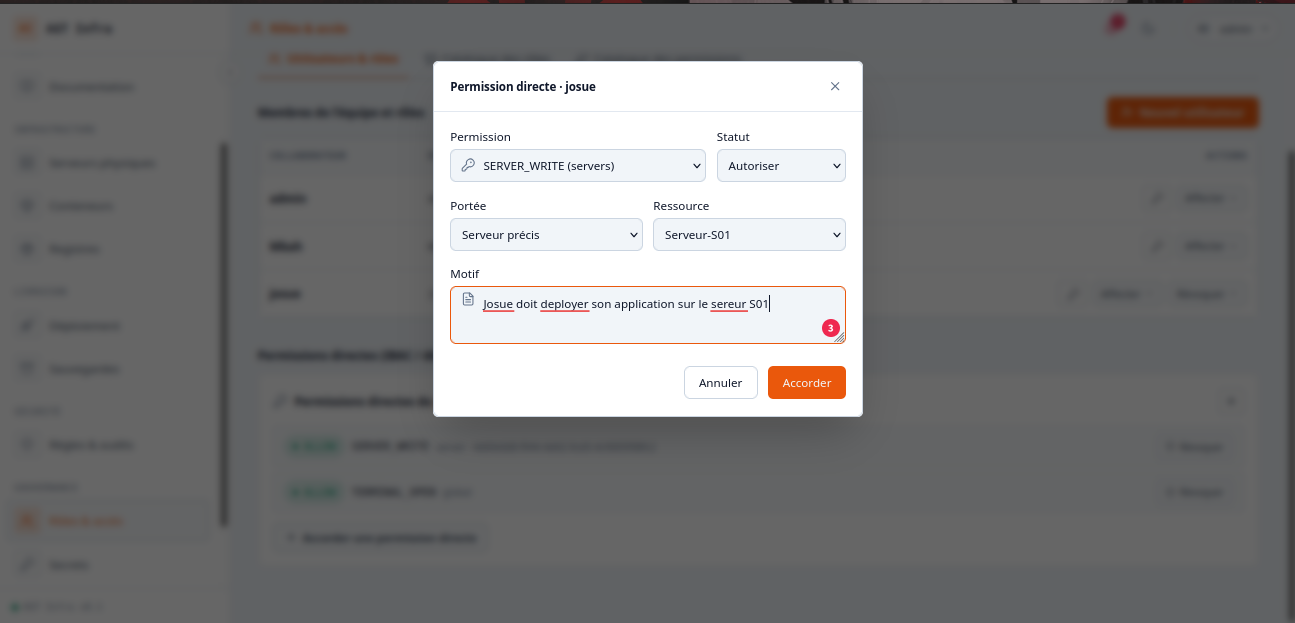
\includegraphics[width=0.7\linewidth]{assets/screenshots/05-screenshot_nouvelle-permission-directe.png}
  \caption{Octroi d'une permission directe scopée à un serveur précis}
\end{figure}

L'écran d'orchestration des déploiements présente l'ensemble des
configurations existantes sous forme de pipelines, chacun rattaché à un
dépôt, une branche, un serveur et un mode d'orchestration (Dockerfile ou
Docker Compose), avec le résultat de sa dernière exécution.

\begin{figure}[H]
  \centering
  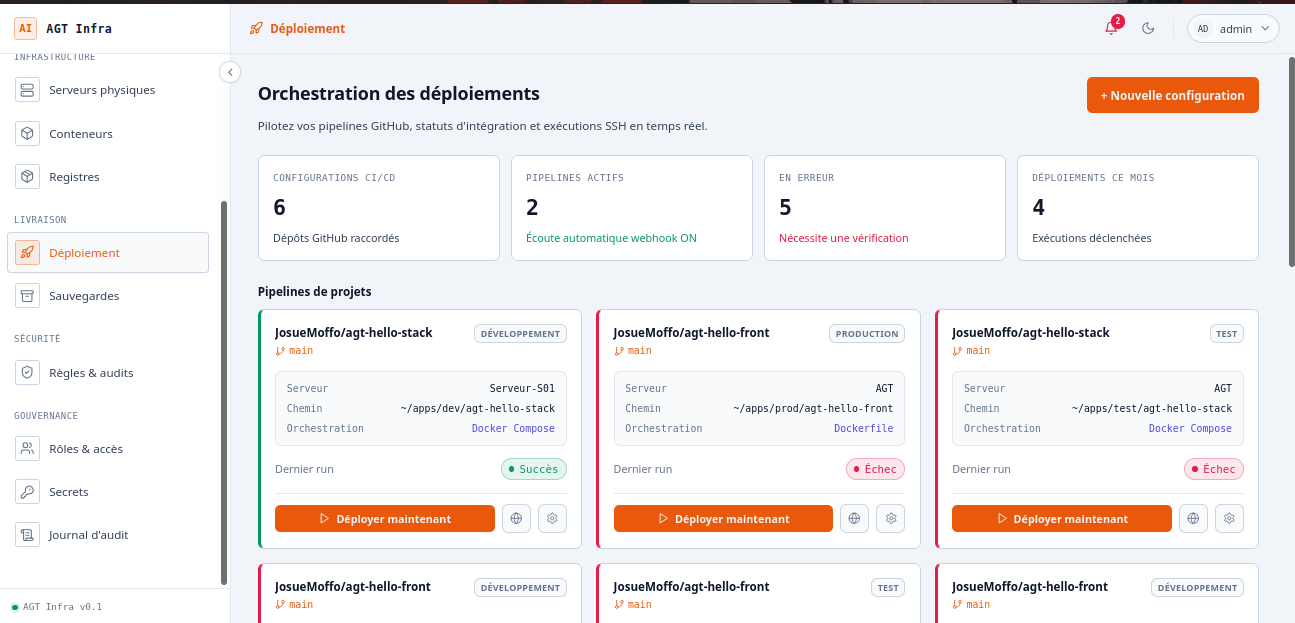
\includegraphics[width=0.85\linewidth]{assets/screenshots/05-screenshot_page-de-deploiement-application.png}
  \caption{Orchestration des déploiements}
\end{figure}

Cette fenêtre correspond au suivi en direct d'un déploiement déclenché
manuellement : les informations de contexte (branche, serveur, durée,
phase en cours) apparaissent en en-tête, tandis que la sortie de chaque
commande exécutée à distance s'affiche au fil de l'eau dans la console.

\begin{figure}[H]
  \centering
  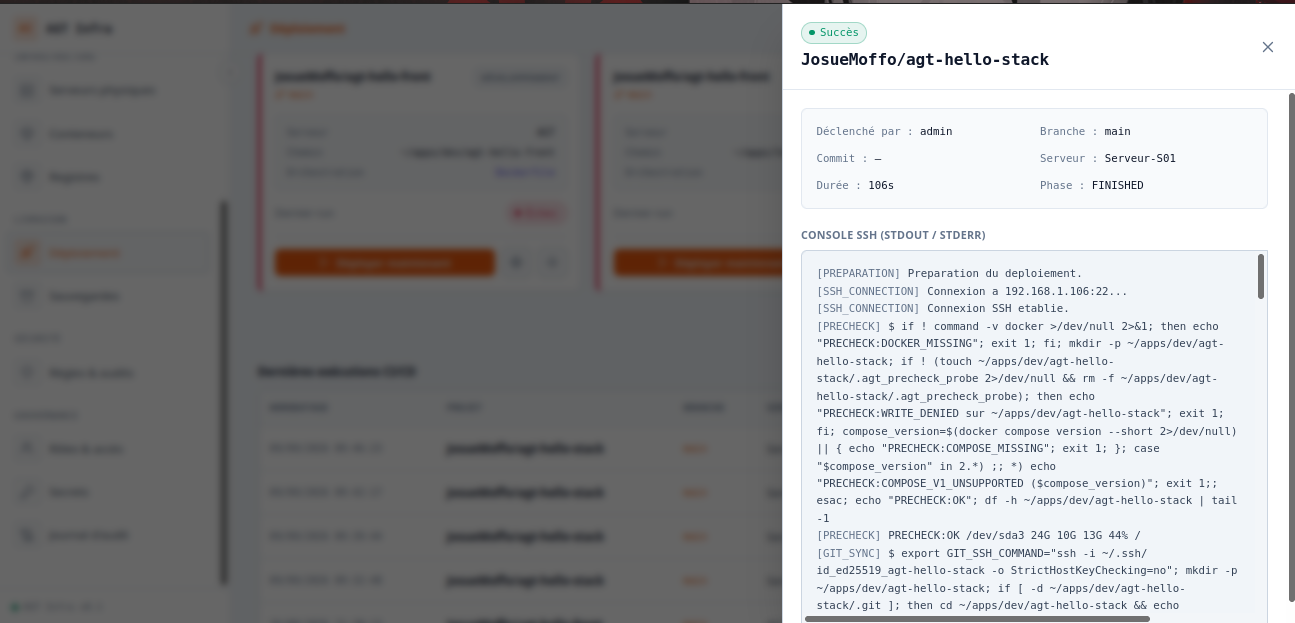
\includegraphics[width=0.7\linewidth]{assets/screenshots/05-screenshot_log-de-deploiement-en-cours.png}
  \caption{Suivi en direct d'un déploiement}
\end{figure}

La fiche détail d'un serveur affiche ses métriques de charge (CPU, RAM,
disque) sous forme de jauges, complétées d'un historique graphique sur
une période choisie, à partir des données collectées à la demande.

\begin{figure}[H]
  \centering
  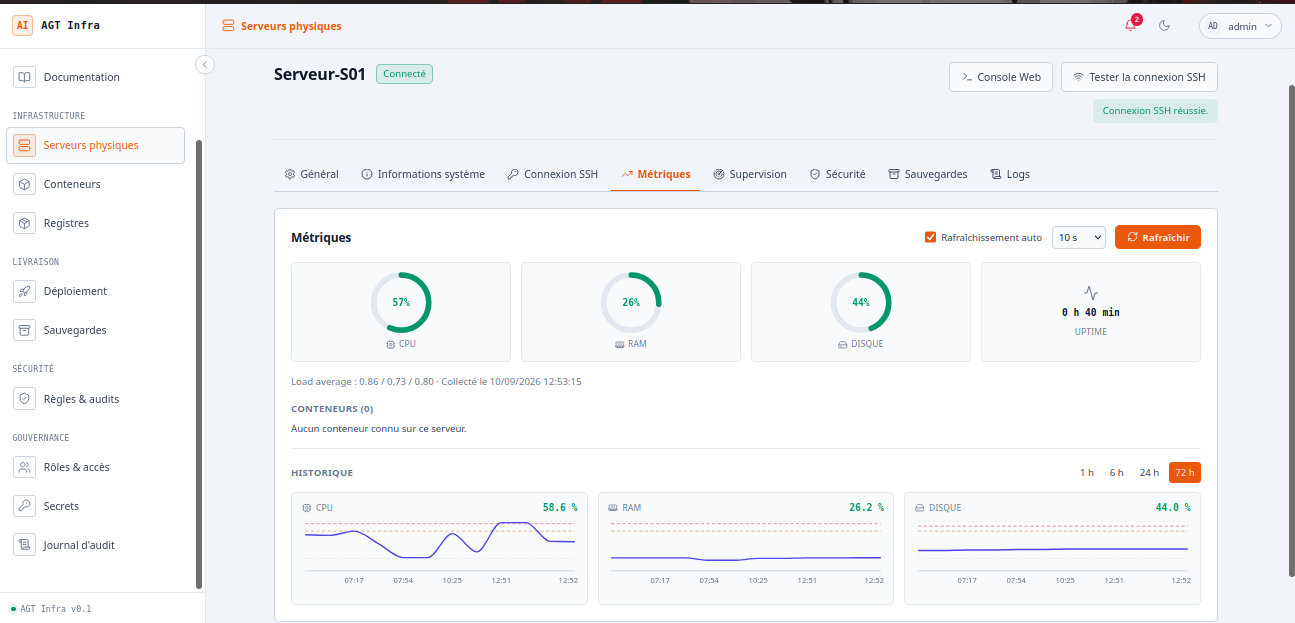
\includegraphics[width=0.85\linewidth]{assets/screenshots/05-screenshot_cllecte-des-metriques.png}
  \caption{Métriques d'un serveur}
\end{figure}

La console web ouvre une session interactive directement depuis
l'interface, sans ouverture d'un client SSH séparé : la capture montre
une session active sur un serveur, avec l'exécution réelle de commandes
système.

\begin{figure}[H]
  \centering
  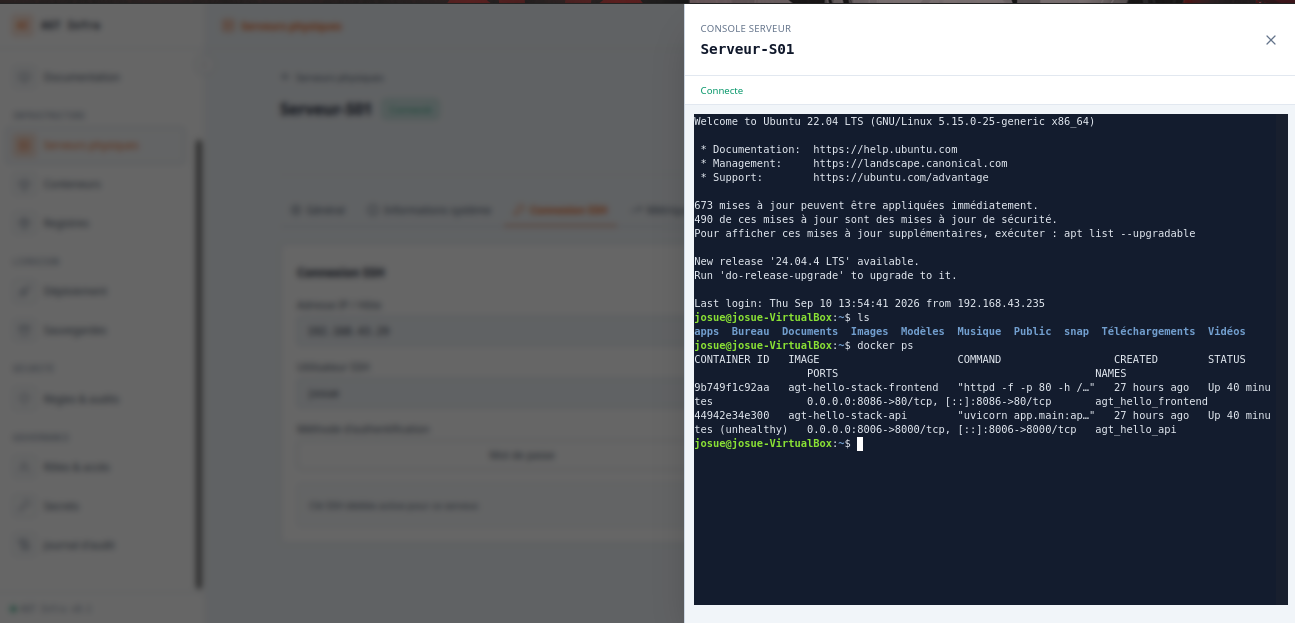
\includegraphics[width=0.7\linewidth]{assets/screenshots/05-screenshot_console-web.png}
  \caption{Console web ouverte sur un serveur}
\end{figure}

Enfin, la documentation intégrée est consultable directement dans
l'interface, organisée par domaine, sans nécessiter de quitter
l'application pour accéder aux prérequis ou aux instructions
d'installation d'un module.

\begin{figure}[H]
  \centering
  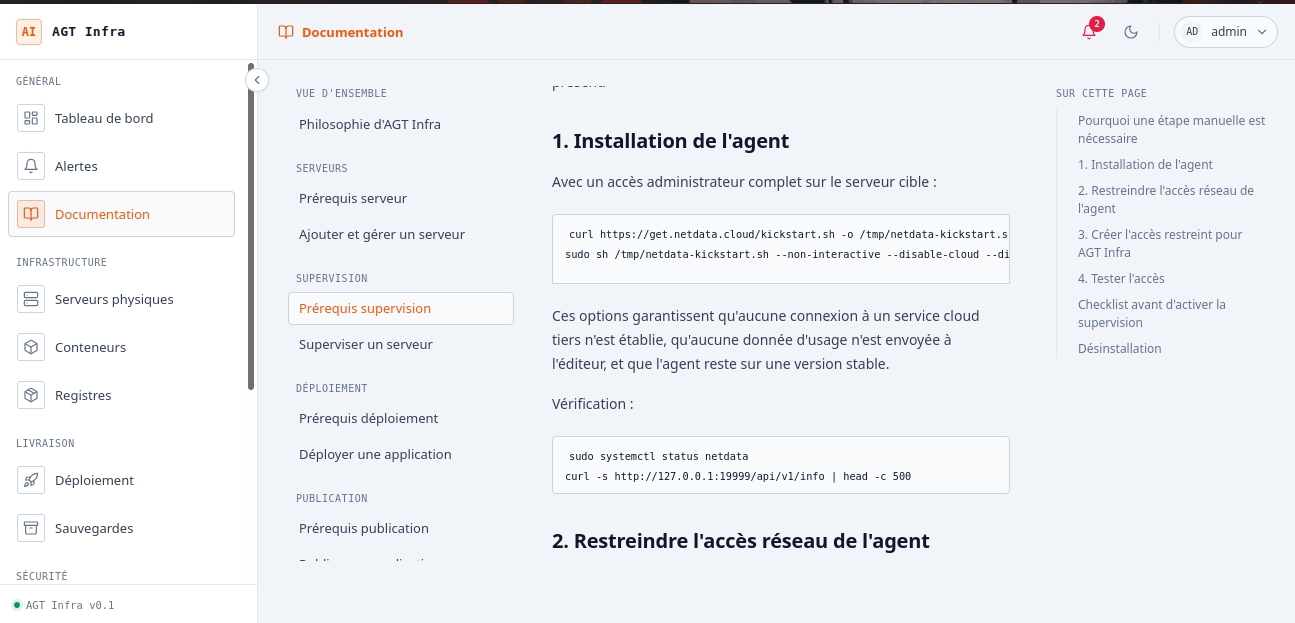
\includegraphics[width=0.85\linewidth]{assets/screenshots/05-screenshot_page-documentation.png}
  \caption{Documentation intégrée}
\end{figure}

\section{Tests et validation}

Le moteur de déploiement a été validé sur deux dépôts créés
spécifiquement pour cette occasion, afin de couvrir les deux modes
d'orchestration de conteneurs pris en charge par AGT Infra : l'un
reposant sur un simple \texttt{Dockerfile}, l'autre sur un
\texttt{docker-compose}. Chacun a été configuré et déployé sur plusieurs
environnements distincts (développement, test, production), avec un
serveur cible réel.

Ces déploiements ont permis de vérifier, en conditions réelles plutôt
que sur simple lecture de code :

\begin{itemize}
  \item la connexion SSH au serveur cible et l'exécution effective des
        huit phases de la séquence de déploiement ;
  \item la diffusion en direct des journaux d'exécution sur le canal
        temps réel dédié ;
  \item la bonne gestion d'un échec de déploiement, sans blocage du
        reste de l'application ;
  \item l'ouverture d'une session de console web sur le serveur cible,
        avec exécution de commandes réelles.
\end{itemize}

\section{Limites actuelles et perspectives}

Plusieurs limites, déjà identifiées au fil des chapitres précédents,
restent assumées à ce jour :

\begin{itemize}
  \item \textbf{Sauvegardes} : aucune sauvegarde automatique des bases
        de données n'est encore implémentée.
  \item \textbf{Montée en charge} : l'ajustement des ressources d'un
        conteneur reste manuel ; aucune réaction automatique à une
        charge excessive n'est prévue à ce stade.
  \item \textbf{Sécurité active} : le moteur de règles de sécurité reste
        à l'état de besoin identifié, non implémenté.
  \item \textbf{Résilience et disponibilité} : chaque serveur reste
        aujourd'hui un point unique de défaillance. Ce point est
        particulièrement sensible pour une application de paiement par exemple, qui ne tolère pas l'indisponibilité.
\end{itemize}

\section{Risques et plans de contournement}

Le tableau~\ref{tab:risques} synthétise les principaux risques déjà
identifiés pour le projet, avec le plan retenu pour en limiter l'impact.

\begin{table}[H]
\centering
\small
\renewcommand{\arraystretch}{1.4}
\begin{tabular}{p{5.5cm}p{8cm}}
\toprule
\textbf{Risque} & \textbf{Plan de contournement} \\
\midrule
Absence de sauvegardes automatiques & Documenter ce manque auprès des
  équipes exploitantes et prioriser ce domaine avant toute mise en
  production d'une application sensible. \\
Exposition de la console web, sans filtrage de contenu & Contrôle
  d'accès strict par permission scopée, enregistrement intégral de
  chaque session. \\
Sécurité des évènements webhook entrants & Vérification systématique de
  la signature avant toute exécution, quel que soit le domaine
  concerné. \\
Gestion manuelle du DNS pour la publication & L'outil guide et vérifie
  la résolution avant de poursuivre, sans jamais automatiser cette
  étape. \\
Dérive de configuration de l'agent de supervision entre serveurs & Guide
  de bootstrap tenu à jour, vérification manuelle recommandée à chaque
  ajout de serveur supervisé. \\
Dépendance à un éditeur tiers pour l'agent de supervision & Limiter la
  dépendance à l'agent lui-même et à son interface documentée. \\
Dépendance aux briques externes pilotées par SSH & Isoler chaque
  intégration derrière un adaptateur dédié, sans jamais bloquer
  l'existant en cas d'erreur. \\
Fuite de secrets (clés SSH, jetons, webhooks) & Chiffrement au repos
  hors du code, isolation par ressource, injection au seul moment de
  l'action. \\
\bottomrule
\end{tabular}
\caption{Risques identifiés et plans de contournement}
\label{tab:risques}
\end{table}